\documentclass[../../main.tex]{subfiles}
\begin{document}

\begin{flushright}
\footnotesize\textit{【自動文字起こし・要確認】}
\end{flushright}

{\bf [解]} 空間座標を設定し，$T$ の4頂点を
\begin{align}
A(0,0,0), \quad B\Bigl(0, \dfrac{1}{\sqrt{2}}, \dfrac{1}{\sqrt{2}}\Bigr), \quad C\Bigl(\dfrac{1}{\sqrt{2}}, 0, \dfrac{1}{\sqrt{2}}\Bigr), \quad D\Bigl(\dfrac{1}{\sqrt{2}}, \dfrac{1}{\sqrt{2}}, 0\Bigr)
\end{align}
とする．平面 $\alpha$ の法線ベクトル $\vec{n} = \begin{pmatrix} a_1 \\ a_2 \\ a_3 \end{pmatrix}$ とする．ただし
\begin{align}
a_1^2 + a_2^2 + a_3^2 = 1, \quad 0 \le a_1, a_2, a_3 \quad \dots \text{①}
\end{align}
として考える．面 $ABC, ACD, ABD, BCD$ を $S_1, S_2, S_3, S_4$ とおくと，$S_1 \sim S_4$ の法線ベクトルは，順に
\begin{align}
\vec{n}_1 &= \begin{pmatrix} 1 \\ -1 \\ -1 \end{pmatrix}, \quad \vec{n}_2 = \begin{pmatrix} -1 \\ 1 \\ -1 \end{pmatrix}, \\
\vec{n}_3 &= \begin{pmatrix} -1 \\ -1 \\ 1 \end{pmatrix}, \quad \vec{n}_4 = \begin{pmatrix} 1 \\ 1 \\ 1 \end{pmatrix}
\end{align}
だから，面 $S_k$ と $\alpha$ のなす角 $\theta_k$ として，
\begin{align}
\cos\theta_1 &= \dfrac{a_1-a_2-a_3}{\sqrt{3}}, \quad \cos\theta_2 = \dfrac{-a_1+a_2-a_3}{\sqrt{3}}, \\
\cos\theta_3 &= \dfrac{-a_1-a_2+a_3}{\sqrt{3}}, \quad \cos\theta_4 = \dfrac{a_1+a_2+a_3}{\sqrt{3}}
\end{align}
だから，求める面積 $S$ として，$T$ の一面の面積 $S_0$ から，
\begin{align}
2S &= \dfrac{\sqrt{3}}{4} \sum_{k=1}^4 |\cos\theta_k| \\
&= \dfrac{1}{4} \Bigl[ |a_1+a_2-a_3| + |a_1-a_2+a_3| + |-a_1+a_2+a_3| + |a_1+a_2+a_3| \Bigr] \quad \dots \text{②}
\end{align}
対称性から，$a_1 \le a_2 \le a_3 \quad \dots \text{③}$ とすると，①とあわせて，
\begin{align}
8S = |a_1+a_2-a_3| + a_1+a_2+3a_3 \quad \dots \text{③}'
\end{align}
である．$a_1+a_2-a_3$ の正負で場合分けする．

\paragraph{$1^\circ \ a_1+a_2 \ge a_3$ の時}
③'から，$8S = 2(a_1+a_2+a_3) \quad \therefore S = \dfrac{1}{4}(a_1+a_2+a_3)$ となる．① $\land$ ③ $\land a_1+a_2 \ge a_3$ を図示して，右図斜線部(境界含む)だから．

平面 $k = a_1+a_2+a_3$ との共有点条件より，

\begin{figure}[htb]
\centering
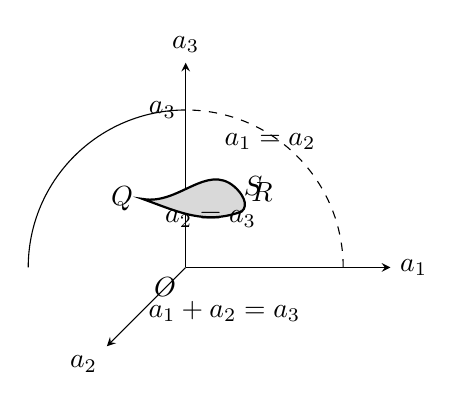
\begin{tikzpicture}[scale=2, >=stealth]
  \draw[->] (0,0,0) -- (1.3,0,0) node[right] {$a_1$};
  \draw[->] (0,0,0) -- (0,1.3,0) node[above] {$a_3$};
  \draw[->] (0,0,0) -- (0,0,1.3) node[below left] {$a_2$};
  
  \coordinate (P) at (0,1,0);
  \coordinate (Q) at (0,0.707,0.707);
  \coordinate (R) at (0.577,0.577,0.577);
  \coordinate (S) at (0.5,0.707,0.5);

  \draw (0,0,0) node[below left] {$O$};
  
  \draw[dashed] (1,0,0) arc (0:90:1);
  \draw (0,1,0) arc (90:180:1);
  
  \draw[thick, fill=gray!30] (Q) to[out=-20,in=200] (R) to[out=40,in=-40] (S) to[out=140,in=-10] cycle;
  
  \node[left] at (P) {$a_3$};
  \node[above right] at (R) {$R$};
  \node[left] at (Q) {$Q$};
  \node[right] at (S) {$S$};
  
  \node[below] at (0.4,0,0.4) {$a_1+a_2=a_3$};
  \node[above right] at (0.3,0.8,0.3) {$a_1=a_2$};
  \node[right] at (0,0.5,0.5) {$a_2=a_3$};
\end{tikzpicture}
\caption{$1^\circ$ における $(a_1,a_2,a_3)$ の存在領域}
\end{figure}

\begin{align}
\begin{cases}
Q \text{で} \min k = \sqrt{2} \\
S \text{で} \max k = \sqrt{3}
\end{cases}
\end{align}
をとり，その間もれ無くとるから，
\begin{align}
\dfrac{\sqrt{2}}{4} \le S \le \dfrac{\sqrt{3}}{4} \quad \dots \text{④}
\end{align}

\paragraph{$2^\circ \ a_1+a_2 \le a_3$ の時}
③'から，$8S = 4a_3 \quad \therefore S = \dfrac{1}{2}a_3$ となる．$1^\circ$ と同様に，$(a_1,a_2,a_3)$ の存在範囲は右図斜線部だから (境界含む)
\begin{align}
\dfrac{1}{\sqrt{6}} \le a_3 \le 1
\end{align}
となり，
\begin{align}
\dfrac{1}{2\sqrt{6}} \le S \le \dfrac{1}{2} \quad \dots \text{⑤}
\end{align}

\begin{figure}[htb]
\centering
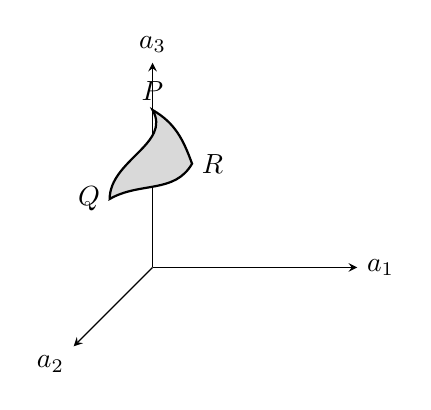
\begin{tikzpicture}[scale=2, >=stealth]
  \draw[->] (0,0,0) -- (1.3,0,0) node[right] {$a_1$};
  \draw[->] (0,0,0) -- (0,1.3,0) node[above] {$a_3$};
  \draw[->] (0,0,0) -- (0,0,1.3) node[below left] {$a_2$};
  
  \coordinate (P) at (0,1,0);
  \coordinate (Q) at (0,0.707,0.707);
  \coordinate (R) at (0.408,0.816,0.408);
  
  \draw[thick, fill=gray!30] (P) to[out=-60,in=90] (Q) to[out=30,in=-120] (R) to[out=110,in=-30] cycle;
  
  \node[above] at (P) {$P$};
  \node[left] at (Q) {$Q$};
  \node[right] at (R) {$R$};
\end{tikzpicture}
\caption{$2^\circ$ における $(a_1,a_2,a_3)$ の存在領域}
\end{figure}

以上④，⑤から，
\begin{align}
\dfrac{1}{2\sqrt{6}} \le S \le \dfrac{1}{2}
\end{align}

\end{document}
